\section{Demo giao diện}
\subsection{Setup môi trường}
Đây là web được xây dựng từ HTML, CSS, JavaScript, PHP và MySQL. Ở đây có Xampp hỗ trợ môi trường để có thể chạy PHP và MySQL.

\begin{figure}[H]
    \centering
    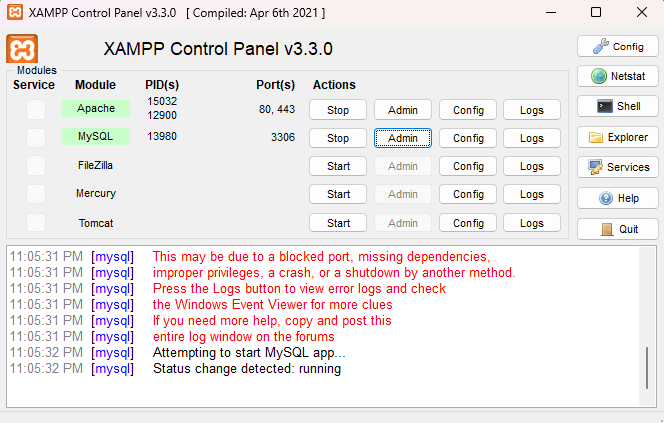
\includegraphics[scale=0.8]{images/xampp.png}
    \caption{Giao diện Xampp}
\end{figure}

Để chạy được PHP có liên kết với MySQL, đầu tiên chúng ta mở ứng dụng XAMPP. Sau đó chúng ta click vào tuần "Start" của Apache và MySQL. Có một lưu ý là nếu chúng ta có một ứng dụng khác chạy trên port "3306" của MySQL xampp đang chạy thì button "Start" sẽ chuyển thành "Stop".

\begin{figure}[H]
    \centering
    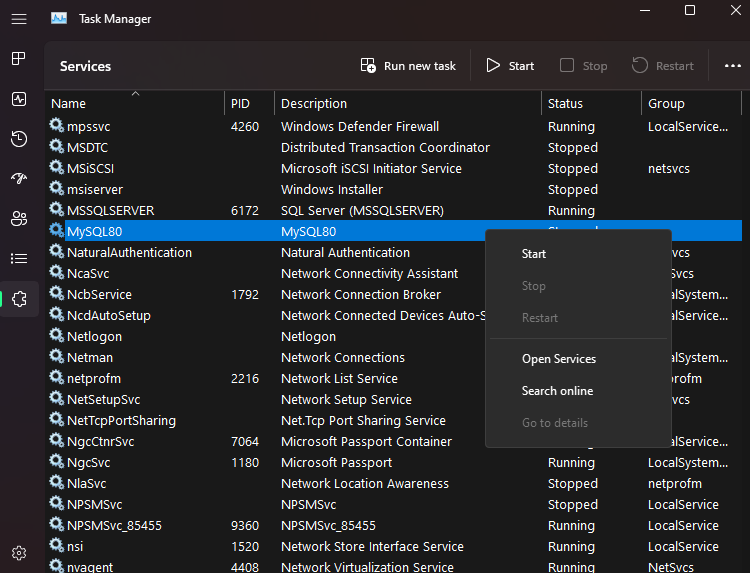
\includegraphics[scale=0.8]{images/taskManager.png}
    \caption{Task Manager}
\end{figure}

Chúng ta chọn vào Service và click chuột phải vào "MySQL80" và chọn "Stop".

\begin{figure}[H]
    \centering
    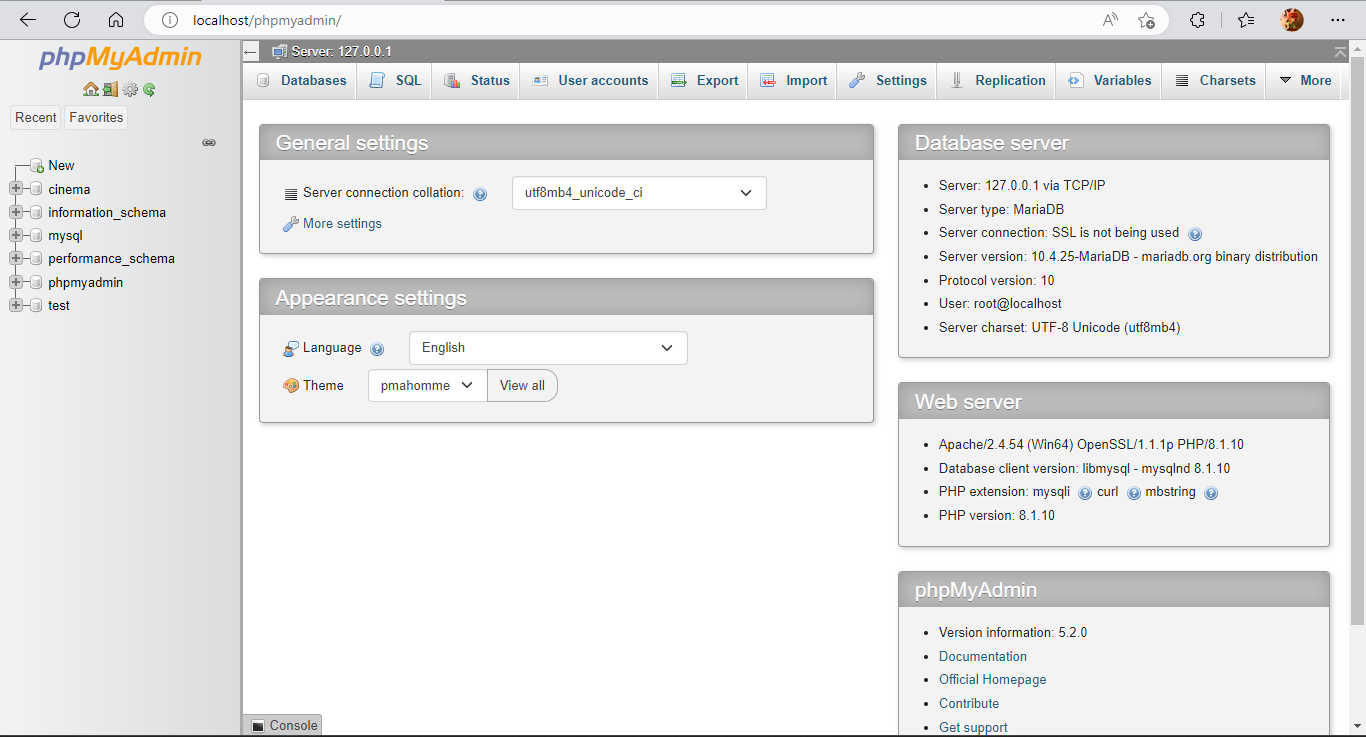
\includegraphics[scale=0.45]{images/phpAdmin.png}
    \caption{Giao diện phpMyAdmin}
\end{figure}
Sau khi MySQL trong XAMPP vẫn giữ trạng thái "Start" thì chúng ta đã khởi động thành công. Sau đó chúng ta click vào "Admin" sau "Start" của MySQL để chúng ta có thể vào giao diện phpMyAdmin.

\subsection{Các chức năng}
- Thêm, sửa và xóa các Customer.\\
- Tìm kiếm các Customer thỏa mãn một hoặc một số điều kiện được nhập vào.\\
- Tìm kiếm Order Food được thanh toán với một số lượng sau một ngày được nhập.\\
- Tìm kiếm ngày đạt được doanh thu được nhập vào trong tháng.\\
- Filter Customer theo giới tính, tổng số điểm tích lũy, theo số đơn hàng mua.\\
- Phân trang cho các sản phẩm có nhiều records.\\
- Sắp xếp theo thứ tự tăng dần hoặc giảm dần của các thuộc tính.\\

\subsection{Hiện thực}
\subsubsection{Home}
\begin{figure}[H]
    \centering
    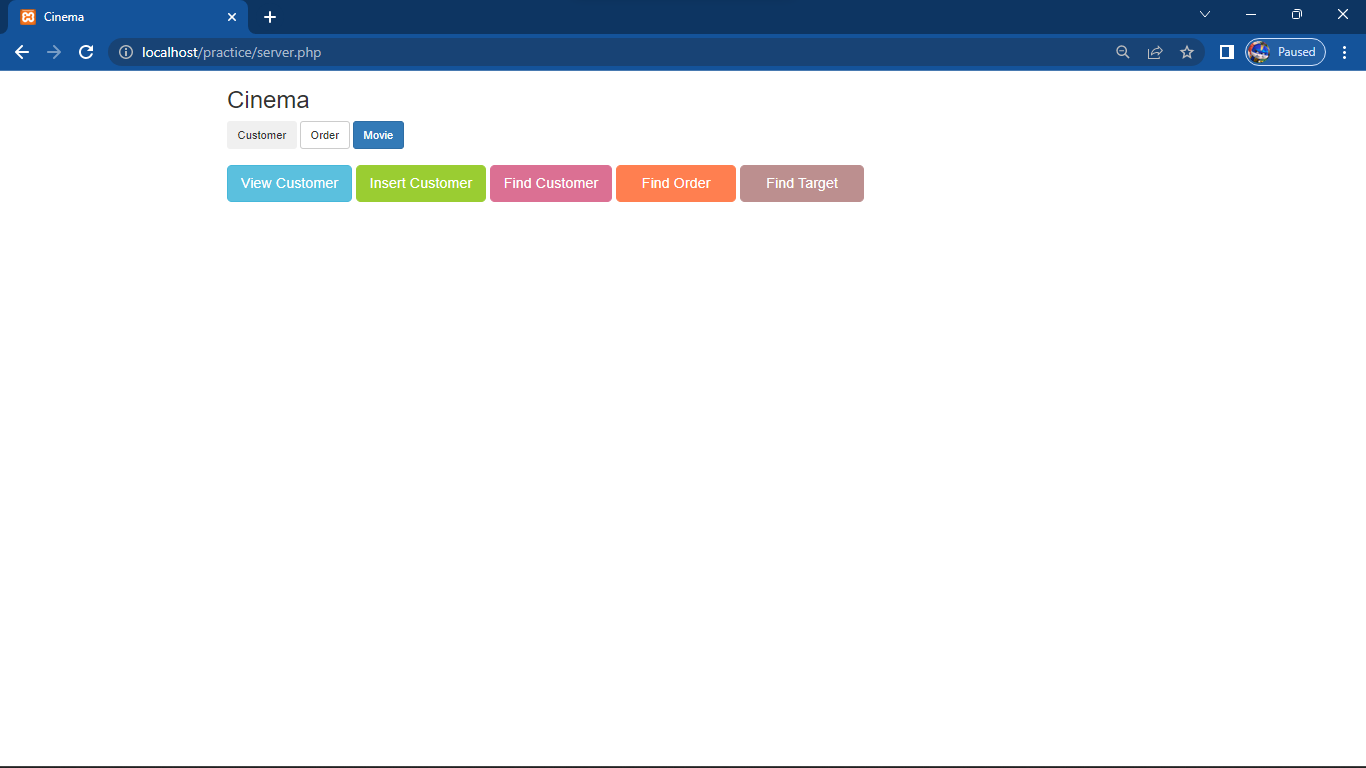
\includegraphics[scale=0.45]{images/viewCustomer.png}
    \caption{Home}
\end{figure}
Ở giao diện này có các đường liên kết điều hướng đến các giao diện khác.

\begin{figure}[H]
    \centering
    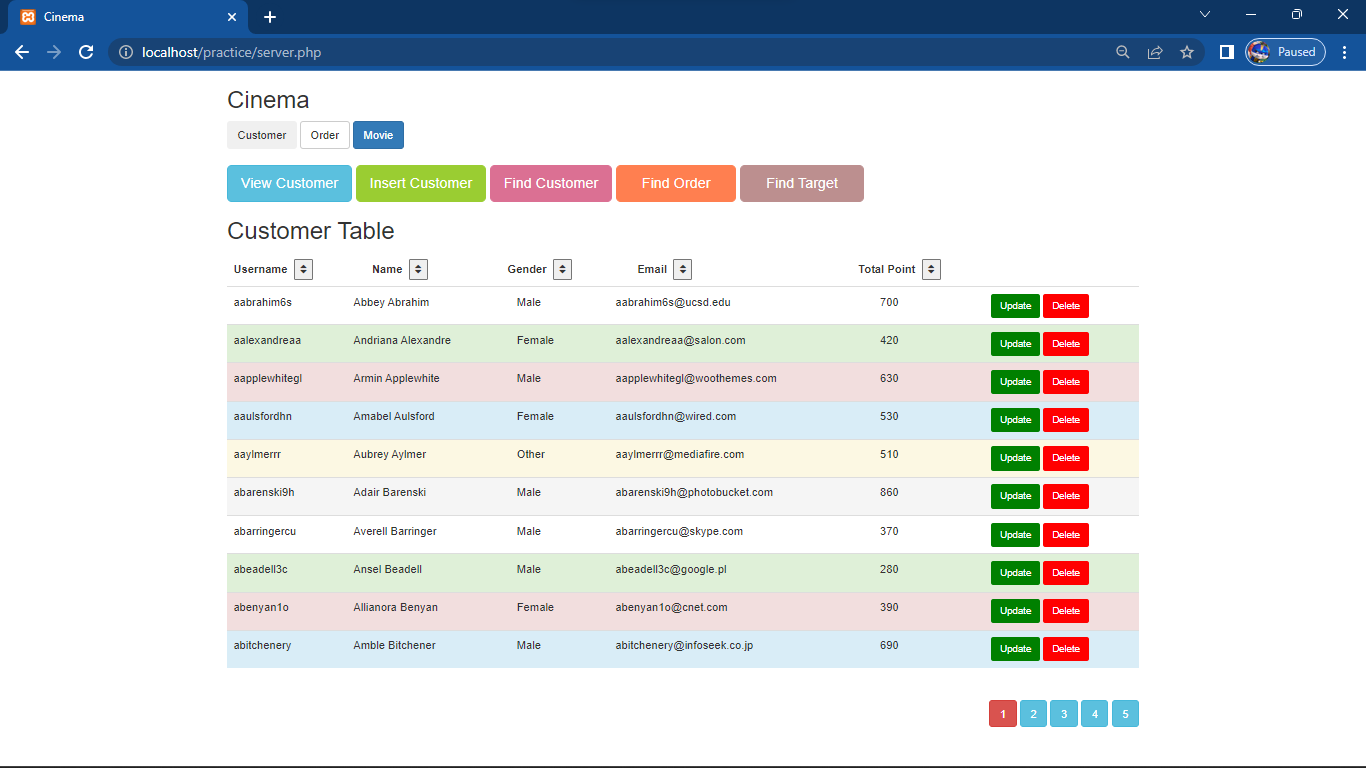
\includegraphics[scale=0.45]{images/viewAll.png}
    \caption{View Customer}
\end{figure}
Khi click vào "view Customer" thì sẽ hiển thị ra giao diện chứa những thông tin về Customer. Trong giao diện này, chúng ta có thể thực hiện các thao tác thêm, sửa và xóa các thông tin liên quan đến Customer. Ở mỗi thuộc tính được hiển thị, chúng ta có thể lựa chọn sắp xếp chúng theo thứ tự tăng hoặc giảm dần.


\subsubsection{Insert Customer}
\begin{figure}[H]
    \centering
    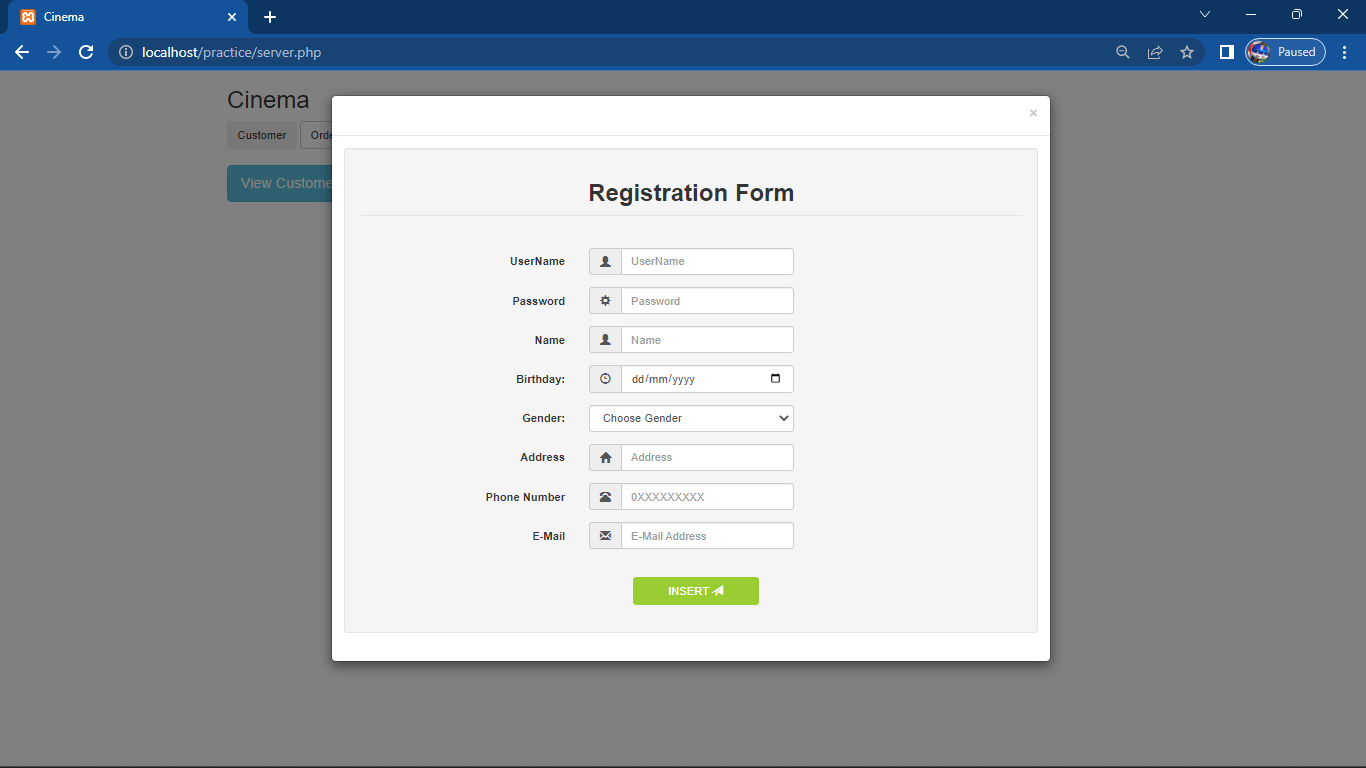
\includegraphics[scale=0.45]{images/insertCustomer.png}
    \caption{Insert Customer}
\end{figure}

Giao diện chứa form cho phép người dùng nhập vào các thông tin của Customer. Ở đây sẽ có validate dữ liệu đầu vào. Ví dụ như format của email, số điện thoại,...

% \subsubsubsection{\textbf{Validate Password}}

\begin{figure}[H]
    \centering
    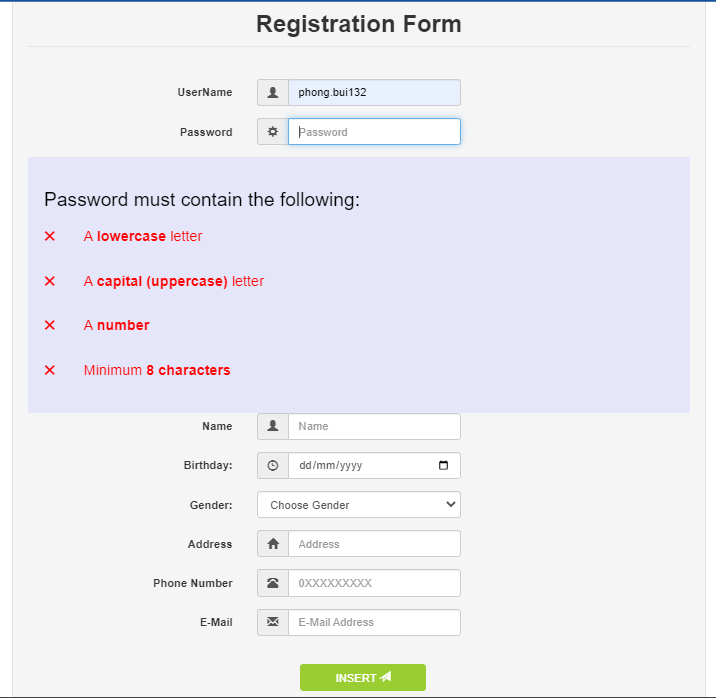
\includegraphics[scale=0.45]{images/insertValidatePassword.png}
    \caption{Validate Password}
\end{figure}
Ở giao diện insert, chúng ta sẽ kiểm tra giá trị nập vào của một số trường. Như ở đây chúng ta kiểm tra giá trị password nhập vào phải chứa cả ký tự in thường, in hoa, số và phải có độ dài hơn từ 8 ký tự trở lên.

\begin{figure}[H]
    \centering
    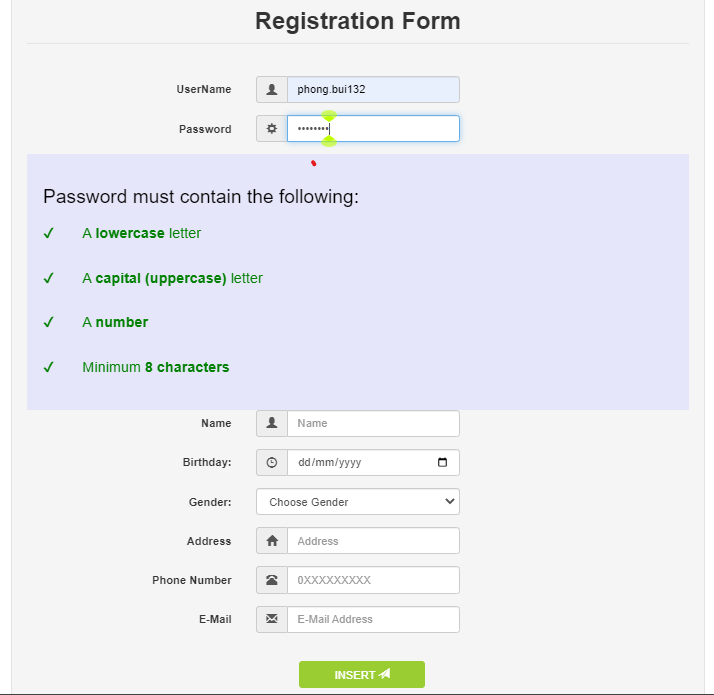
\includegraphics[scale=0.45]{images/insertValidateRightPassword.png}
    \caption{Validate Password}
\end{figure}
Khi input được nhập thì sẽ những điều kiện sẽ hiển thị màu xanh ở những điều kiện thoải mãn.

\begin{figure}[H]
    \centering
    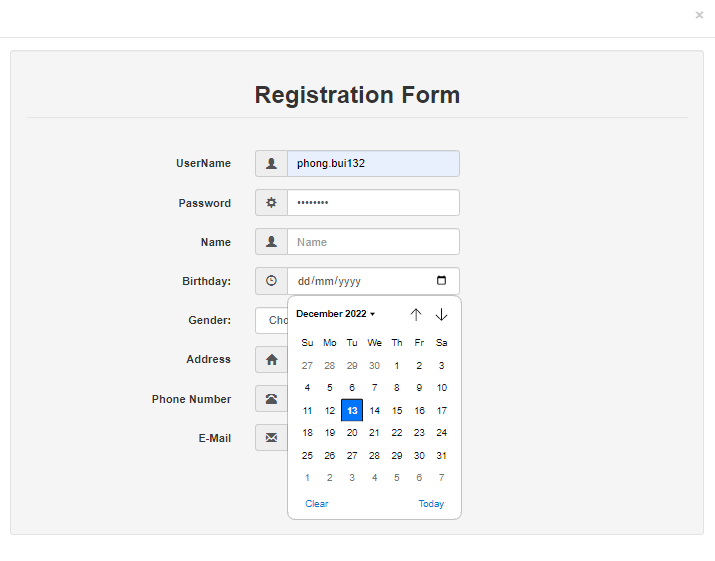
\includegraphics[scale=0.45]{images/calendarPicker.png}
    \caption{Calendar picker}
\end{figure}
Khi chọn vào trường Birthday để nhập thì calendar picker sẽ được hiển thị để người dùng chọn.

\begin{figure}[H]
    \centering
    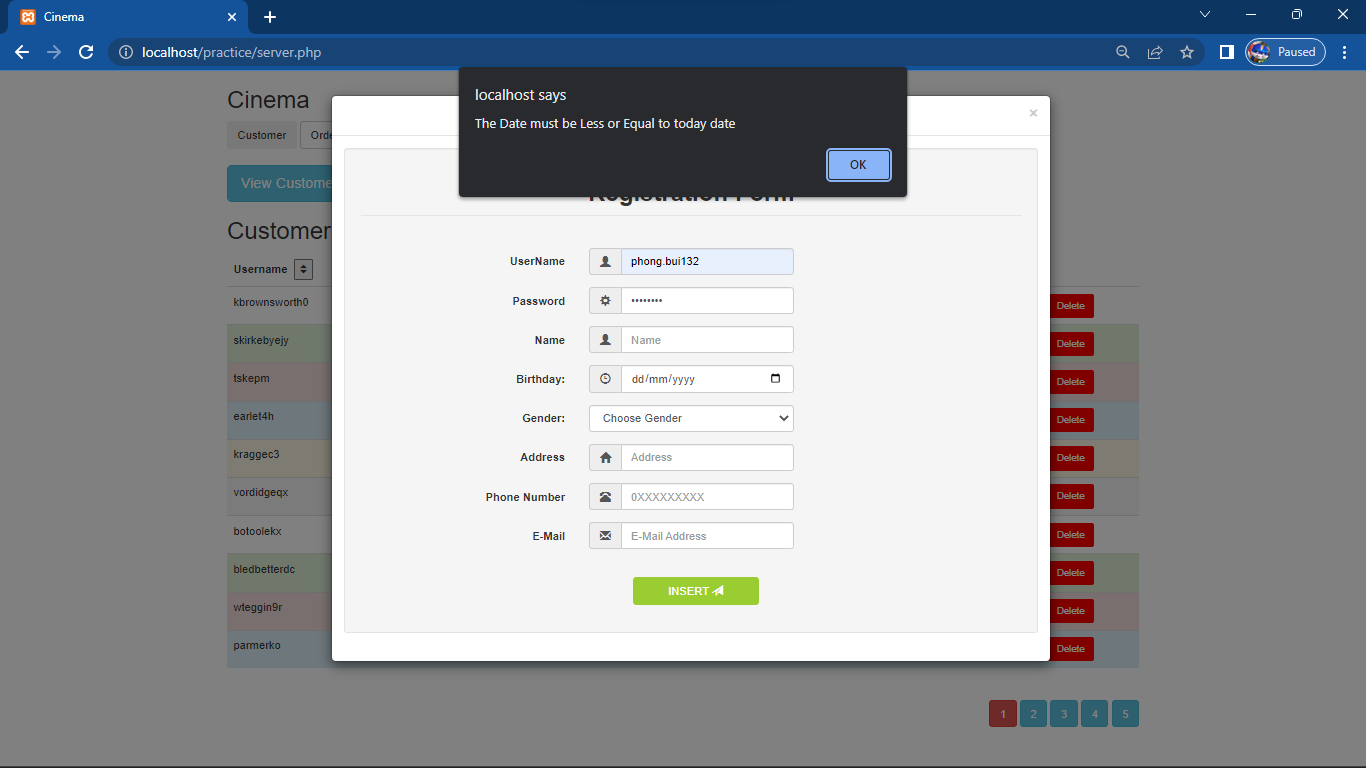
\includegraphics[scale=0.45]{images/validateBirthday.png}
    \caption{Validate Birthday}
\end{figure}
Nếu ngày được chọn lớn hơn ngày ở hiện tại thì sẽ có thông báo được hiện ra về việc input Birthday không hợp lệ.

\begin{figure}[H]
    \centering
    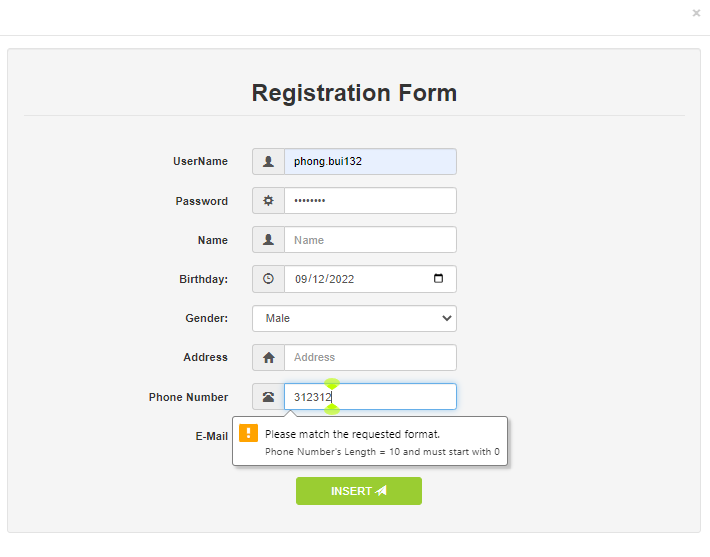
\includegraphics[scale=0.45]{images/validatePhone.png}
    \caption{Validate Phone Number}
\end{figure}
Format được dùng cho Phone Number là phải bắt đầu bằng "0" và độ dài phải là 10 số. Nếu nhập sai sẽ có thông báo hiển thị.

\begin{figure}[H]
    \centering
    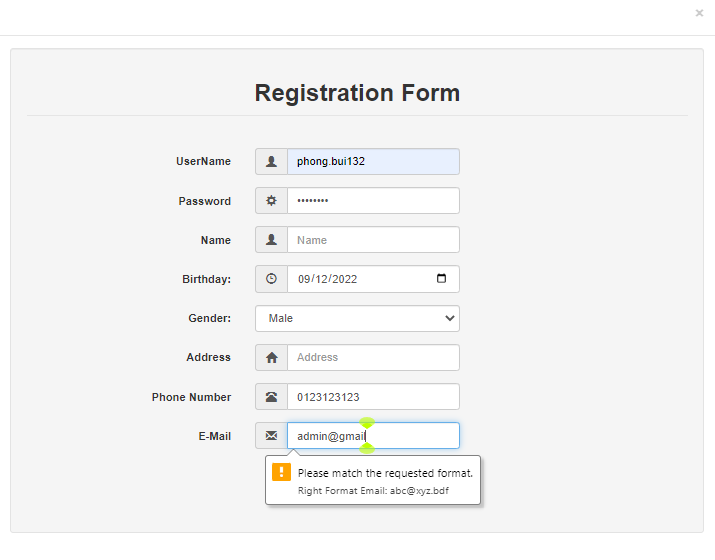
\includegraphics[scale=0.45]{images/validateEmail.png}
    \caption{Validate Email}
\end{figure}
Format của email sẽ là "abc@xyz.bdf". Nếu không có "@" hoặc sau "@xyz." không có thì sẽ báo lỗi.
\begin{figure}[H]
    \centering
    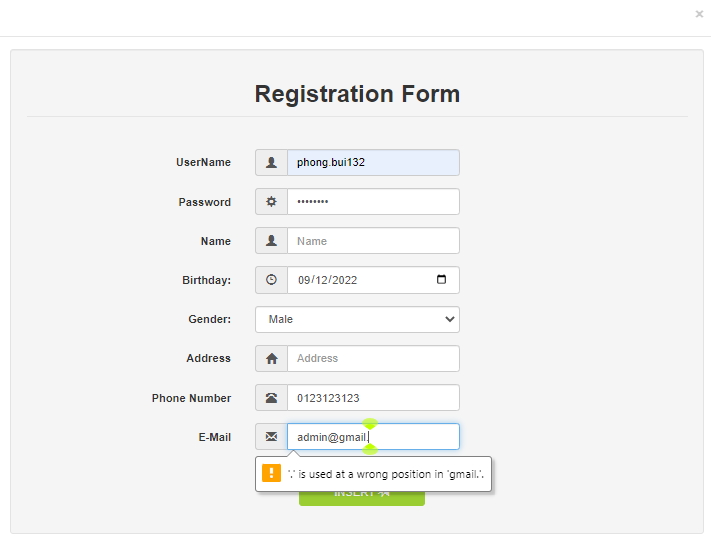
\includegraphics[scale=0.45]{images/validateEmail_02.png}
    \caption{Validate Email}
\end{figure}


\subsubsection{Search Information}
\begin{figure}[H]
    \centering
    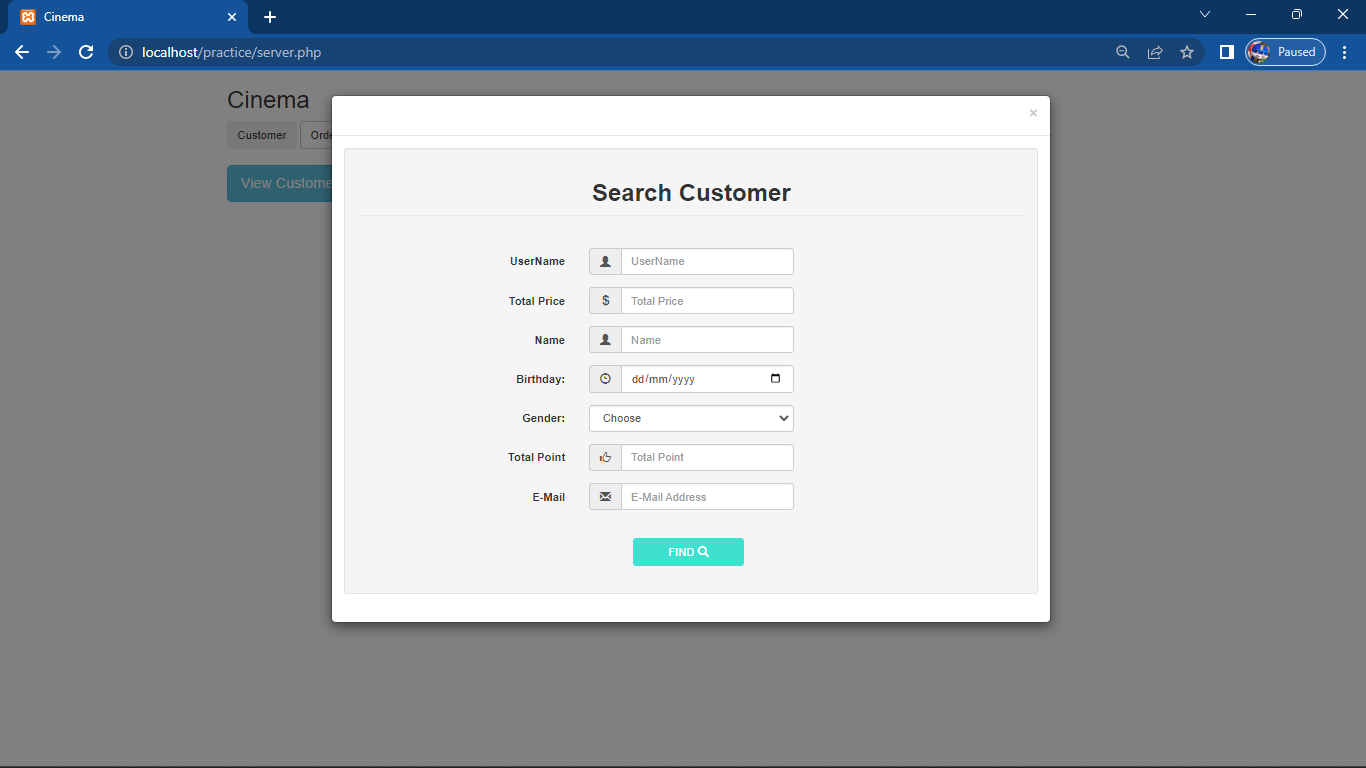
\includegraphics[scale=0.45]{images/searchAndFilter_Customer.png}
    \caption{Search Information About Customer}
\end{figure}
Giao diện chứa form có thể nhập một số thông tin để tìm kiếm. Như muốn tìm kiếm một Customer nào đó chúng ta có thể nhập vào Username hoặc Name hoặc email của họ. Nếu chúng ta chỉ chọn Gender thì kết quả sẽ lọc ra những Customer có giới tính là Gender đã chọn. Nếu nhập vào Total Price thì sẽ lọc ra những Customer có tổng giá trị đơn hàng đã mua từ giá trị đã nhập trở lên.

\subsubsection{Find Order}
\begin{figure}[H]
    \centering
    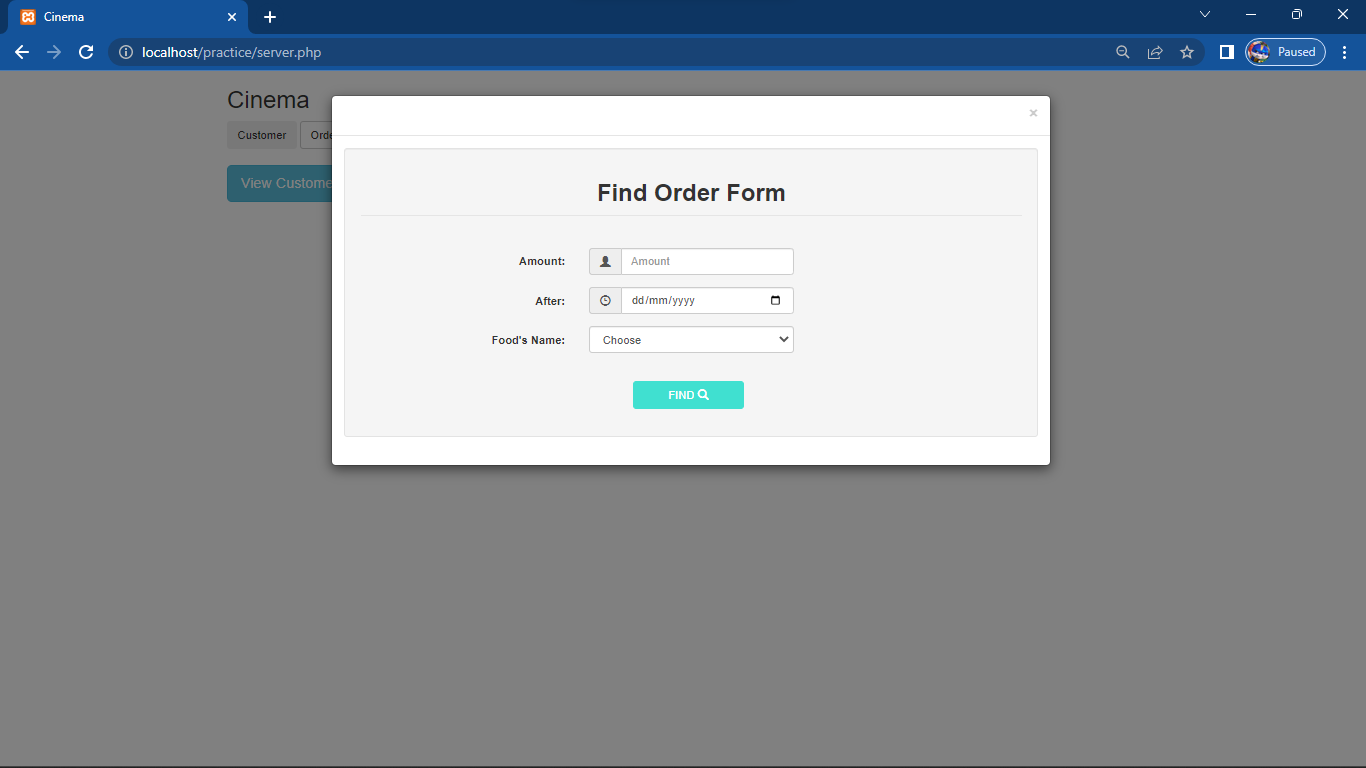
\includegraphics[scale=0.45]{images/findOrder.png}
    \caption{Find Order}
\end{figure}
Giao diện này cho phép chúng ta tìm những đơn hàng Food với một số lượng nhất định sau ngày mà chúng ta đã chọn.


\subsubsection{Find Date Reach Target}
\begin{figure}[H]
    \centering
    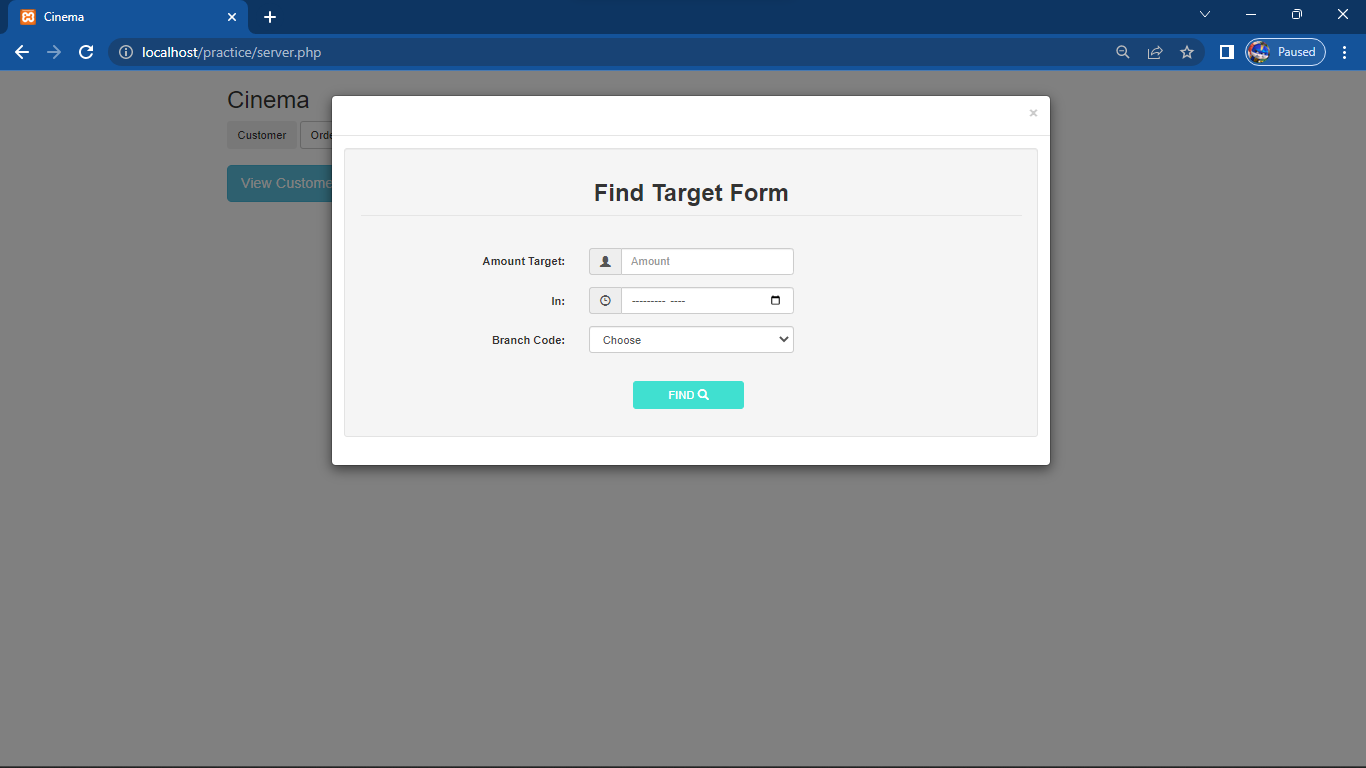
\includegraphics[scale=0.45]{images/findDateReachTarget.png}
    \caption{Find Date Reach Specific Target}
\end{figure}

Giao diện này giúp chúng ta tìm được ngày mà chúng ta đạt doanh thu đề ra trong tháng.

